% ---- Modele TP PC V2 -----------
\documentclass[a4paper,9pt,french]{scrartcl}
\usepackage[T1]{fontenc}%---pour l'encodage d'entr\'ee
\usepackage{array}%---pour les tableaux
\usepackage{titlesec}%---modification des titres
\usepackage{ulem}%---pour le soulignage
\usepackage[dvipsnames]{xcolor}%---pour avoir d'autres couleurs
\usepackage{color}%---pour avoir les couleurs de base
\usepackage{babel}%---pour les trucs de langue et la francisation

\usepackage{graphicx}%----pour mettre des images
\usepackage[utf8]{inputenc}%---encodage
\usepackage{geometry}%---pour modifier les tailles et mettre a4paper
%\usepackage{awesomebox}%---pour les boites d'exercices, de pbq et de croquis ---d\'esactiv\'e pour les TP de PC
\usepackage{tikz}%---pour dessiner + d\'ependance de chemfig
%\usepackage{tabularx}%---pour dimensionner automatiquement les tableaux avec variable X
\usepackage{fancyhdr}%---pour les en-t\^ete personnalis\'ees
\usepackage{blindtext}%---pour les liens
\usepackage{hyperref}%---pour les liens (\`a mettre en dernier)
\usepackage{caption}%---pour la francisation de la l\'egende table vers Tableau
 \usepackage{float}% --- pour placer les figures et tableaux où l'on souhaite avec argument H
 \usepackage{multicol}
 \usepackage{amsmath}
 \usepackage{geometry}
 \geometry{vmargin=2.5cm}

\captionsetup{labelfont=sc}%---pour la francisation de la l\'egende table vers Tableau
\def\frenchtablename{Tableau}%---pour la francisation de la l\'egende table vers Tableau
\pagestyle{fancy}
\renewcommand\headrulewidth{1pt}
\fancyhead[L]{TP 3}
\fancyhead[R]{Saux Paulhenry}
\title{Compte rendu de TP 3}
\date{}
\author{}

\geometry{a4paper}
% ----------- Création des commandes de couleur ----------
\makeatletter
\newcommand{\coloruline}[2]{%
        \UL@protected\def\temp@uline{\leavevmode \bgroup
            \markoverwith{\textcolor{#1}{\rule[-0.5ex]{2pt}{0.4pt}}}%
        \ULon}%
        \temp@uline{#2}%
    }

    \newcommand{\coloruuline}[2]{%
        \UL@protected\def\temp@uuline{\leavevmode \bgroup
            \UL@setULdepth
            \ifx\UL@on\UL@onin \advance\ULdepth2.8\p@\fi
            \markoverwith{\textcolor{#1}{\lower\ULdepth\hbox
                {\kern-.03em\vbox{\hrule width.2em\kern1\p@\hrule}\kern-.03em}}}%
        \ULon}%
        \temp@uuline{#2}%
    }

\makeatother

\renewcommand{\thesection}{\arabic{section}}
\renewcommand{\thesubsection}{\arabic{subsection}}
\renewcommand{\thesubsubsection}{\arabic{subsubsection}}
\begin{document}
% ---------------- Modification des titres de niveau 1,2 et 3 --------------------
\titleformat
{\section} % command
%[display] % shape
{\Large} % format
{\coloruuline{red}{\thesection. }} % label
{0ex} % sep
{\coloruuline{red}} % before-code
[] % after-code

\titleformat
{\paragraph} % command
%[display] % shape
{\Large} % format
{\coloruline{NavyBlue}{\theparagraph. }} % label
{0ex} % sep
{\coloruline{NavyBlue}} % before-code
[] % after-code

\titleformat
{\subsection} % command
%[display] % shape
{\Large} % format
{\coloruline{red}{\thesection.\thesubsection. }} % label
{0ex} % sep
{\coloruline{red}} % before-code
[] % after-code

\titleformat
{\subsubsection} % command
%[display] % shape
{\large} % format
{\coloruline{ForestGreen}{\thesection.\thesubsection.\thesubsubsection. }} % label
{0ex} % sep
{\coloruline{ForestGreen}} % before-code
[] % after-code

\titleformat
{\chapter} % command
%[display] % shape
{\large} % format
{\coloruline{NavyBlue}{\thechapter \:- }} % label
{0ex} % sep
{\coloruline{NavyBlue}} % before-code
[] % after-code


% ---------------- Début du corps du document ------------------------------------

\section{Introduction}
L'objectif de ce TP est d'étudier le comportement réel d'un fluide (SF6) lors d'une compression isotherme. Il s'agit de :
\begin{itemize}
    \item  Mettre en évidence le phénomène de transition de phase (liquéfaction).
   \item  Tracer les isothermes d'Andrews dans le diagramme de Clapeyron (P,V).
    \item Identifier les domaines d'existence des phases (gaz, liquide, équilibre liquide-vapeur).
    \item Observer l'influence de la température sur  l'étendue du palier de liquéfaction.
\end{itemize}

   
\section{Protocole}
\subsection{Matériel}
\begin{itemize}
    \item manomètre
    \item Enceinte transparente contenant du SF6 et du mercure donc le volume de ce dernier est réglable
    \item Enceinte contenant la première remplie d'eau
    \item Régulateur de température de l'eau
\end{itemize}
\subsection{Description du montage expérimental}
Le dispositif utilise une cellule contenant une masse fixe de SF6. Le tube est plongé dans un bain thermostaté (eau) pour maintenir une température T constante.

Un volant permet d'élever une colonne de mercure qui agit comme un piston, réduisant ainsi le volume V du gaz. On relève la pression P via un manomètre pour chaque volume V imposé (graduations sur le tube).

On attend 2 à 3 minutes après chaque changement de volume pour que l'équilibre thermique soit atteint.
\begin{center}
%
\includegraphics[scale=0.3]{circuit1}
\end{center}
\subsection{Mesures à effectuer}
On effectue 2 séries de mesure, l'une avec T=25°C et l'autre avec T=35°C. Dans les 2 cas, le protocole est le m\^eme :
\begin{enumerate}
    \item Placer le volume à 4 cm$^3$
    \item Attendre 2min.
    \item Relever la pression, ainsi que l'état du fluide.
    \item Par pas de 0.5 cm$^3$, refaire les étapes 2 et 3 jusqu'à atteindre une pression de 50 bar.
    \item Refaire les mesures pour un volume inférieur de 0.25 au volume de changement d'état du fluide, cette fois par pas de 0.1 jusqu'à observer le changement d'état. 
    \item Replacer le volume à 4cm$^3$.
\end{enumerate}
\section{Mesures}
\subsection{Données}
% \begin{table}[H]
%     \begin{center}
%         \begin{tabular}{lll}
% V (cm$^3$) & P ($10^5$ Pa)& Présence de fluide liquide \\
% 4,00    & 14,0    & Non                        \\
% 3,75 & 14,0    & Non                        \\
% 3,5  & 15,5 & Non                        \\
% 3,25 & 16,0    & Non                        \\
% 3,00   & 17,0    & Non                        \\
% 2,75 & 18,0    & Non                        \\
% 2,5  & 19,5  & Non                        \\
% 2,25 & 21,0    & Non                        \\
% 2,00    & 22,5  & Non                        \\
% 1,95 & 23,0    & Non                        \\
% 1,90  & 23,0    & Non                        \\
% 1,85 & 23,5 & Oui                        \\
% 1,80  & 23,5 & Oui                        \\
% 1,75 & 23,5  & Oui                        \\
% 1,50  & 23,5  & Oui                        \\
% 1,25 & 24,0    & Oui                        \\
% 1,00    & 24,0    & Oui                        \\
% 0,75 & 24,5  & Oui                        \\
% 0,50  & 25,0    & Oui                        \\
% 0,35 & 48,0    & Oui                        
% \end{tabular}
%     \end{center}
% \caption{Évolution de la pression en fonction du volume pour une températeure fixée à 25°C.}
% \end{table}

% \begin{table}[H]
%     \begin{center}
%      \begin{tabular}{lll}
% V (cm³) & P (10⁵ Pa) & Présence de fluide à l’état liquide \\
% 4       & 14         & Non                                 \\
% 3,75    & 14,5       & Non                                 \\
% 3,5     & 15,5       & Non                                 \\
% 3       & 18         & Non                                 \\
% 2,5     & 20         & Non                                 \\
% 2,25    & 22         & Non                                 \\
% 2       & 23,5       & Non                                 \\
% 1,75    & 25,5       & Non                                 \\
% 1,7     & 25,5       & Non                                 \\
% 1,6     & 26         & Non                                 \\
% 1,55    & 26         & Oui                                 \\
% 1,5     & 26,5       & Oui                                 \\
% 1       & 27         & Oui                                 \\
% 0,5     & 28         & Oui                                 \\
% 0,35    & 48         & Oui                                 \\                                 
% \end{tabular}   
%     \end{center}
% \caption{Évolution de la pression en fonction du volume pour une températeure fixée à 30$^\circ$ C.}

% \end{table}


\begin{table}[H]
    \centering
    \small
    \begin{tabular}{|c||lc|lc|}
    \hline
    \textbf{Volume} & \multicolumn{2}{c|}{\textbf{Série 1 : $25^\circ C$}} & \multicolumn{2}{c|}{\textbf{Série 2 : $30^\circ C$}} \\ 
    \cline{2-5}
    $V \text{ (cm}^3\text{)}$ & $P \text{ (10}^5\text{ Pa)}$ & \textbf{Liq ?} & $P \text{ (10}^5\text{ Pa)}$ & \textbf{Liq ?} \\ 
    \hline
    4,00 & 14,0 & Non & 14,0 & Non \\
    3,75 & 14,0 & Non & 14,5 & Non \\
    3,50 & 15,5 & Non & 15,5 & Non \\
    3,25 & 16,0 & Non & --   & --  \\
    3,00 & 17,0 & Non & 18,0 & Non \\
    2,75 & 18,0 & Non & --   & --  \\
    2,50 & 19,5 & Non & 20,0 & Non \\
    2,25 & 21,0 & Non & 22,0 & Non \\
    2,00 & 22,5 & Non & 23,5 & Non \\
    1,95 & 23,0 & Non & --   & --  \\
    1,90 & 23,0 & Non & --   & --  \\
    1,85 & 23,5 & Oui & --   & --  \\
    1,80 & 23,5 & Oui & --   & --  \\
    1,75 & 23,5 & Oui & 25,5 & Non \\
    1,70 & --   & --  & 25,5 & Non \\
    1,60 & --   & --  & 26,0 & Non \\
    1,55 & --   & --  & 26,0 & Oui \\
    1,50 & 23,5 & Oui & 26,5 & Oui \\
    1,25 & 24,0 & Oui & --   & --  \\
    1,00 & 24,0 & Oui & 27,0 & Oui \\
    0,75 & 24,5 & Oui & --   & --  \\
    0,50 & 25,0 & Oui & 28,0 & Oui \\
    0,35 & 48,0 & Oui & 48,0 & Oui \\
    \hline
    \end{tabular}
    \caption{Évolution de la pression en fonction du volume pour une températeure fixée à 25$^\circ$ C et 30$^\circ$ C.}
\end{table}
\subsection{Incertitudes}

L'évaluation des incertitudes de mesure sur la pression $P$ et le volume $V$ est réalisée  en considérant que l'erreur de lecture est liée à la graduation minimale des instruments.

Le tube gradué présente une division tous les $0,05 \text{ cm}^3$. En considérant une erreur de lecture égale à une demi-graduation, l'incertitude-type $u(V)$ est donnée par :
\begin{equation}
    u(V) = \frac{0,05}{\sqrt{3}} \approx 0,03 \text{ cm}^3
\end{equation}
Le manomètre est gradué tous les $1 \text{ bar}$ (soit $1 \times 10^5 \text{ Pa}$). De la même manière, l'incertitude-type $u(P)$ liée à la lecture est :
\begin{equation}
    u(P) = \frac{1}{\sqrt{3}} \approx 0,6 \text{ bar}
\end{equation}
Bien que les incertitudes de lecture soient prédominantes, d'autres facteurs peuvent influencer la précision des résultats :
\begin{itemize}
    \item Un temps d'attente insuffisant après la compression peut entraîner une surestimation de la pression (échauffement adiabatique).
     \item Une fluctuation de la température du bain marie impacte la pression de vapeur saturante. 
\end{itemize}
\section{Graphiques}
\begin{figure}[H]
 \begin{center}
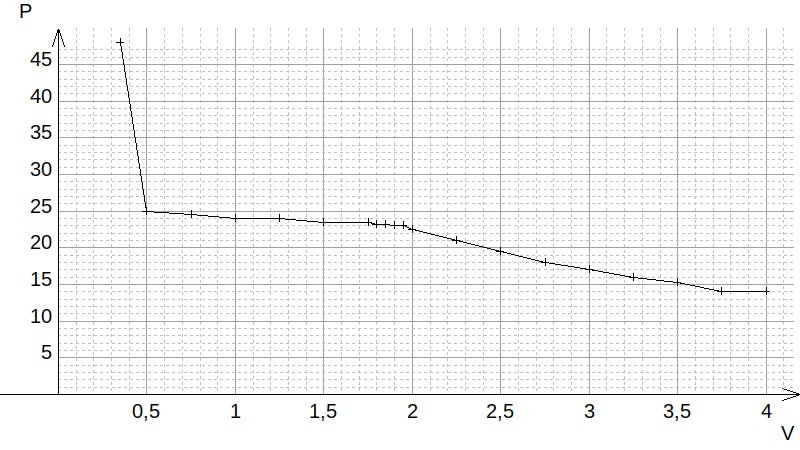
\includegraphics[scale=0.4]{g1}
 \end{center}
\caption{Évolution de la pression en fonction du volume pour une températeure
fixée à 25$^\circ$C.}
\end{figure}

\begin{figure}[H]
 \begin{center}
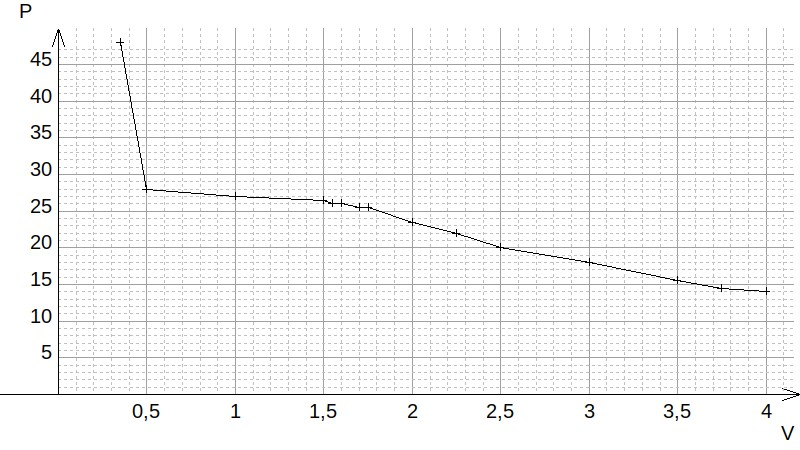
\includegraphics[scale=0.4]{g2}
 \end{center}
\caption{Évolution de la pression en fonction du volume pour une températeure
fixée à 30$^\circ$C.}
\end{figure}
\begin{figure}[H]
 \begin{center}

\includegraphics[scale=0.6]{c1}
 \end{center}
\end{figure}
\begin{figure}[H]
 \begin{center}

\includegraphics[scale=0.6]{c2}
 \end{center}
\end{figure}
\section{Exploitation des résultats}
\subsection{Étude de l'isotherme}
%TODO GRAPHE 1/V
On observe 3 parties distinctes sur le graphique : une augmentation progressive 
de la pression, un plateau et une augmentation brutale de la pression. Ces trois zones sont 
à mettre e relation avec l'état du fluide observé. Lors de l'augmentation progressive,
ce dernier est à l'état gazeux, puis à partir de l'état saturant et durant tout le plateau, il est
en transition de phase. Enfin, quand il ne reste plus du fluide à l'état liquide, la pression augmente brutalement.

L'évolution de la pression durant l'intervalle de changement de phase est la somme de deux phénomènes. Nous diminuons le volume, donc la pression augmente. Cela provoque la condensation du fluide, qui prend alors moins de place.
La pression diminue donc. Il y a donc un équilibre entre le volume et le titre en vapeur qui permet de maintenir la 
pression constante.

Concernant la première phase où le fluide est gaz, on peut tenter de la modéliser comme si il se comportait comme un gaz parfait.
On a alors
\begin{equation}
    PV = nRT = Cst
\end{equation}
On peut vérifier la relation avec quelques valeurs obtenues :

\begin{table}[]
    \begin{center}
\begin{tabular}{lll}
V (cm$^3$) & P ($10^5$ Pa) & PV (Unité arbitraire) \\
4,00       & 14,0       & 56,0                   \\
3,00       & 17,0       & 51,0                   \\
2,00       & 22,5       & 45,0                   \\
1,90       & 23,0       & 43,7                                     
\end{tabular}
\end{center}
\end{table}

Pour vérifier si l'écart à la loi des gaz parfaits est significatif, on calcule l'incertitude relative sur le produit $PV$ :
\begin{equation}
    \frac{u(PV)}{PV} = \sqrt{\left(\frac{u(P)}{P}\right)^2 + \left(\frac{u(V)}{V}\right)^2}
\end{equation}

Pour le point à $4,00 \text{ cm}^3$ ($P=14,0$ bar) :
\begin{itemize}
    \item $\frac{u(P)}{P} = \frac{0,29}{14} \approx 2,1 \%$
    \item $\frac{u(V)}{V} = \frac{0,014}{4} \approx 0,35 \%$
\end{itemize}
On obtient une incertitude élargie $U(PV) = 2 \times u(PV) \approx 2,4$.

La chute de la valeur de $PV$ (de $56,0$ à $43,7$, soit un écart de $12,3$) est très largement supérieure à l'incertitude de mesure ($2,4$). On en conclut que le $SF_6$ s'écarte de manière indiscutable du modèle du gaz parfait dans ces conditions de pression.

La pression réelle est plus faible que celle prédite par la loi des gaz parfaits ; ce n'est donc pas un gaz parfait.
\subsection{Effet de l'augmentation de la température}

La comparaison des deux séries de mesures permet de mettre en évidence l'influence de la température sur l'équilibre liquide-vapeur.

À $25^\circ C$, le palier de liquéfaction (transition de phase) se situe environ à $23,5 \times 10^5 \text{ Pa}$. 

À $30^\circ C$, ce palier remonte à environ $26,0 \times 10^5 \text{ Pa}$. La pression de saturation est donc une fonction croissante de la température.

Le début de la condensation se produit à un volume plus faible lorsque la température augmente (passage de $1,90 \text{ cm}^3$ à $1,60 \text{ cm}^3$ environ). Le gaz doit être davantage comprimé pour amorcer la transition à haute température.

De plus, On observe que l'étendue du volume sur lequel on observe un état diphasiqe diminue avec l'augmentation de la température.


La donnée à $T_c = 45,6^\circ C$ indique l'existence d'une température critique. À cette température précise,
le palier de transition de phase disparaît totalement. De plus, la distinction physique entre la phase liquide et la phase vapeur s'estompe : les masses volumiques des deux phases deviennent identiques.

\subsection{Représentation dans un diagramme}
On a représenter les points de transition de phase des 2 séries de mesures.

Pour le fréon, avec le diagramme de Mollier, on trouve les couples (p,T), pour la transition de phase vapeur/liquide :
(6 ,20), (8 ,30), (10, 40), (15,50) et (40, 100) environ pour le point critique. On le représente de la m\^eme façon.

On remarque que pour une température ambiante de $30^\circ C$, la pression de vapeur saturante du $SF_6$ ($26 \times 10^5$ Pa) est plus de trois fois supérieure à celle du Fréon ($8 \times 10^5$ Pa). Le $SF_6$ est donc un fluide beaucoup plus volatil.

La température critique du Fréon ($100^\circ C$) est nettement supérieure à celle du $SF_6$ ($45,6^\circ C$). 
En conséquence, le Fréon permet des cycles de changement de phase sur une plage thermique plus large, ce qui peut justifier son utilisation comme fluide frigorigène dans le TP IV.

\section{Conclusion}

Ce TP a permis de caractériser expérimentalement le comportement réel du $SF_6$ à travers 
l'étude des isothermes d'Andrews dans le diagramme de Clapeyron. 
L'observation du palier de pression constante lors de la compression a mis
 en évidence l'équilibre liquide-vapeur et a permis de vérifier que la pression
  de vapeur saturante est une fonction croissante de la température. 

Par ailleurs, l'étude du produit $PV$ a démontré que 
le modèle du gaz parfait est insuffisant pour décrire le fluide 
à haute pression, les interactions intermoléculaires devenant 
prédominantes à l'approche de la liquéfaction. Enfin, nous avons constaté que
 l'augmentation de la température réduit l'étendue du domaine diphasique, 
 illustrant la convergence des phases liquide et vapeur vers le point critique.
\end{document}
